
\documentclass[
	% -- opções da classe memoir --
	12pt,				% tamanho da fonte
	oneside,			% para impressão em verso e anverso. Oposto a oneside
	a4paper,			% tamanho do papel. 
	brazil				% o último idioma é o principal do documento
	]{abntex2}

% ---
% Pacotes básicos 
% ---
\usepackage{fontspec}
\usepackage{longtable}
\setmainfont{Arial}
\usepackage[top=2cm, bottom=2cm, left=2cm, right=2cm]{geometry}
\usepackage[utf8]{inputenc}		% Codificacao do documento (conversão automática dos acentos)
\usepackage{indentfirst}		% Indenta o primeiro parágrafo de cada seção.
\usepackage{color}				% Controle das cores
\usepackage{graphicx}			% Inclusão de gráficos
\usepackage{microtype} 			% para melhorias de justificação
\usepackage{multicol}			% multiplas colunas no texto
\usepackage{graphicx,url}
\usepackage{float}
\usepackage{slashbox}
% ---

% ---
% Pacotes de citações
% ---
\usepackage[brazilian]{backref}	 % Paginas com as citações na bibl
\usepackage[alf]{abntex2cite}	% Citações padrão ABNT
\usepackage{indentfirst}
% --- 
% CONFIGURAÇÕES DE PACOTES
% --- 

% ---
% Configurações do pacote backref
% Usado sem a opção hyperpageref de backref
\renewcommand{\backrefpagesname}{Citado na(s) página(s):~}
% Texto padrão antes do número das páginas
\renewcommand{\backref}{}
% Define os textos da citação
\renewcommand*{\backrefalt}[4]{
	}%
% ---

% ---
% Informações de dados para CAPA e FOLHA DE ROSTO

% ---


% ---
% Configurações de aparência do PDF final

% alterando o aspecto da cor azul
\definecolor{blue}{RGB}{41,5,195}

% informações do PDF
\makeatletter
\hypersetup{
     	%pagebackref=true,
		pdftitle={\@title}, 
		pdfauthor={\@author},
    	pdfsubject={\imprimirpreambulo},
	    pdfcreator={LaTeX with abnTeX2},
		colorlinks=true,       		% false: boxed links; true: colored links
    	linkcolor=black,          	% color of internal links
    	citecolor=black,        		% color of links to bibliography
    	filecolor=magenta,      		% color of file links
		urlcolor=black,
		bookmarksdepth=4
}
\makeatother
% --- 

% --- 
% Espaçamentos entre linhas e parágrafos 
% --- 

% O tamanho do parágrafo é dado por:
\setlength{\parindent}{1.3cm}

% Controle do espaçamento entre um parágrafo e outro:
\setlength{\parskip}{0.2cm}  % tente também \onelineskip

% ---
% compila o indice
% ---
\makeindex
% ---

% ----
% Início do documento
% ----
\begin{document}

% Seleciona o idioma do documento (conforme pacotes do babel)
%\selectlanguage{english}
\selectlanguage{brazil}

% Retira espaço extra obsoleto entre as frases.
\frenchspacing 

% ----------------------------------------------------------
% ELEMENTOS PRÉ-TEXTUAIS
% ----------------------------------------------------------
% \pretextual



% ---
% Capa
% ---
%%%%%%%%%%%%%%%%   CAPA   %%%%%%%%%%%%%%%%%%%%%%      
%\begin{document} 



%\begin{titlepage}
\begin{center}

\begin{figure}[!htb]
%\centering

\includegraphics[width=1.1\textwidth]{USFCAR_-_logo.jpg}\

\end{figure}


\vspace{80pt}
\LARGE{\textbf{Bacharelado Ciência da Computação}}\\
\LARGE{Tema 2}\\
\LARGE{ }

\vspace{50pt}
\textbf{\Huge{}}

\end{center}
	
\begin{flushleft}
		
\begin{center}
{\Large 	Grupo 5\\
			 Aléssia Melo - 620289\\
			 Caio Henrique Giacomelli - 620297\\
  			 Gabriela Ramos - 620360\\
  			 Matheus Augusto Thomaz - 620599\\}
\end{center}
        
\vspace{70pt}

 \begin{center}

{\large { Maio / 2017 \\Bancos de Dados e Engenharia de Software II e WEB } \\
Profª Drª Sahudy Montenegro González\\
Profª Drª Luciana Zaina \\
Profº Drº Alexandre Álvaro} 
                    
\end{center}
        
\end{flushleft}	
  
%\end{titlepage}



% ---


% ---
% inserir o sumario
% ---
\pdfbookmark[0]{\contentsname}{toc}
\tableofcontents*
\cleardoublepage
% ---



% ----------------------------------------------------------
% ELEMENTOS TEXTUAIS
% ----------------------------------------------------------
\textual

% ----------------------------------------------------------
% Introdução (exemplo de capítulo sem numeração, mas presente no Sumário)
% ----------------------------------------------------------

% ----------------------------------------------------------



% ----------------------------------------------------------
% Apresentamos o texto
% ----------------------------------------------------------
\chapter{Escopo}
\section{Objetivo}
	Neste documento será descrito o gerenciamento do projeto cujo o objetivo é desenvolver uma aplicação web que realiza consultas sob uma simulação da base de dados do IMDb (Internet Movie Database), que é uma coleção de informações de filmes disponível na web.
    
    
   A aplicação possibilitará buscas avançadas de atores, que incluem o nome, intervalo de anos ou ano específico de filmes em que trabalhou, sexo e nome do personagem e também em quais filmes o ator X e o ator Y trabalharam juntos. 
   
   
   Além disso, constam neste documento o escopo do produto, EAP (Estrutura Analítica do Projeto), cronograma e plano de risco. 
   
\section{Descrição}
O sistema a ser desenvolvido será uma aplicação Web capaz de realizar consultas relacionadas a base de dados do IMBb, para isso, também contará com um sistema de paginação para possibilitar a exibição dos dados a serem retornados. Portanto, o sistema será composto por duas consultas principais:
 
\begin{itemize}

\item \textbf{Consulta 1:} trata-se de uma busca avançada de atores, que incluem o nome, intervalo de anos ou ano específico de filmes em que trabalhou, sexo e nome do personagem. Tal consulta será decomposta em:
\begin{itemize}
\item\textit{ Subconsulta 1:} Consulta de atores por sexo, nome relativo do personagem e ano específico em que estes trabalharam;
\item \textit{Subconsulta 2:} Consulta de atores por nome e intervalo de anos;
\end{itemize}
\item \textbf{Consulta 2:} trata-se de uma busca simples que correlacione dois atores e retorne os filmes em que estes trabalharam juntos.
\end{itemize}

Todas as consultas citadas retornarão algumas informações relacionadas aos atores, contendo título e ano do filme em que contracenaram, nome e sexo do ator, assim como o nome do personagem que este realizou. Outrossim, a consulta 2 será ordenada lexicograficamente pelos nomes dos atores.

\chapter{Requisitos}
\section{Funcionais}
RF1: O sistema deverá permitir a consulta de ator por nome, sendo esta uma busca absoluta, e intervalo de anos em que este trabalhou.

RF2: O sistema deverá permitir a consulta de atores por sexo, nome de personagem, sendo esta uma busca relativa, e ano específico de filme.

RF3: O sistema deverá permitir a consulta que correlaciona dois atores e retorne os filmes em que estes trabalharam juntos.

RF4: O sistema deverá exibir o resultado da consulta, referente ao requisito funcional 3, em forma de lista
ordenada lexicograficamente por nome dos atores.


\section{Não-Funcionais}

RNF1: O sistema será desenvolvido na linguagem de programação \textit{Java}.

RNF2: O sistema deverá ser compatível com o navegador \textit{Chrome}.

RNF3: O SGDB usado deve ser o 
\textit{PostgreSQL}.

RNF4: A interface gráfica deverá ser implementada em \textit{HTML} e \textit{CSS}.

\chapter{EAP}
\section{Dicionário}
\textbf{Escopo:} Descreve os processos necessários para se alcançar os resultados esperados no desenvolvimento do projeto.

\textbf{EAP:} Estrutura Analítica de Projetos ou em inglês WBS (Work Breakdown Structure) é utilizada para evidenciar as entregas do projeto, o que auxuliará na gestão do escopo do projeto. 

\textbf{MVC:} Model-view-controller é um padrão de arquitetura de software (design pattern) que separa a aplicação em 3 camadas. A camada de interação do usuário(view), a camada de manipulação dos dados(model) e a camada de controle(controller).

\section{Diagrama}
\begin{figure}[htb]
%\centering
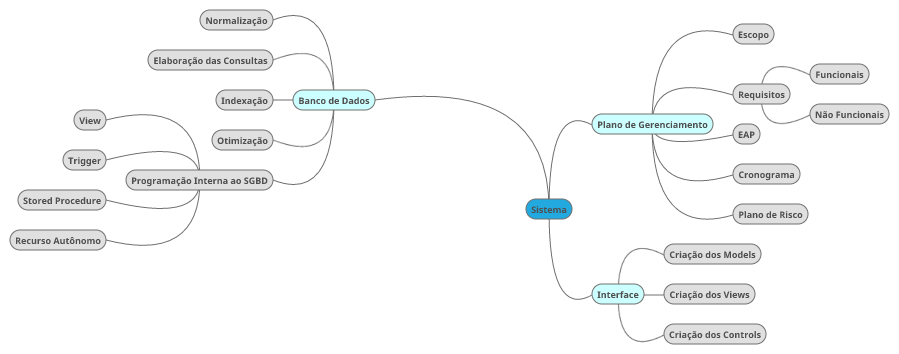
\includegraphics[width=1.05\textwidth]{diagrama.png}\
\caption{\label{fig: diagrama}Diagrama EAP}
\end{figure}

\chapter{Cronograma}
A seguir será apresentado o cronograma com as estimativas de datas para realizar as atividades a serem entregues.


\begin{figure}[htb]
%\centering
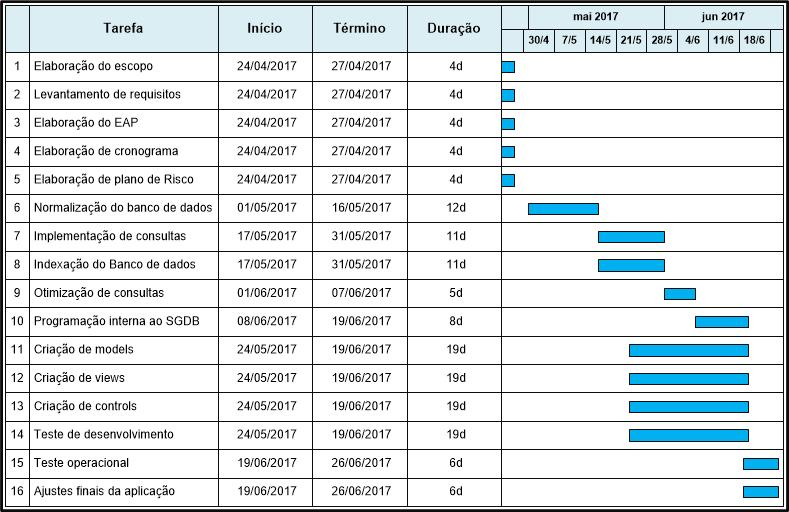
\includegraphics[width=1.05\textwidth]{Cronograma.jpg}\
\caption{\label{fig: cronograma}Cronograma de Atividades}
\end{figure}

\chapter{Plano de Riscos}
\section{Identificação dos Riscos}
 
\begin{center}
\begin{tabular}{|l|*{4}{c|}}\hline
\makebox[3em]{\textbf{Risco}}&\makebox[5em]{\textbf{Descrição}}&\makebox[8em]{\textbf{Probabilidade}}&\makebox[5em]{\textbf{Impacto}}\\\hline\hline

1 & Mudança de requisitos & Alta & Moderado\\\hline
2 & Mudança de escopo & Baixa & Alto \\\hline
3 & Escassez de tempo & Média & Moderado \\\hline
4 & Inexperiência da equipe & Média & Alto \\\hline
5 & Dificuldades com ferramentas & Alta & Moderado \\\hline
6 & Sobrecarga de trabalho & Baixa & Moderado \\\hline
\end{tabular}
\end{center}

\section{Monitoramento e Controle de Riscos}
\begin{center}
\begin{tabular}{|l|*{4}{c|}}\hline
\makebox[3em]{\textbf{Risco}}&\makebox[5em]{\textbf{Monitoramento}}&\makebox[10em]{\textbf{Medidas para Controle}}\\\hline\hline

1 & Reuniões com os docentes envolvidos & Validação ou remoção do requisito em questão
\\\hline
2 & Reuniões com os docentes envolvidos & Negociação em relação à mudança \\\hline
3 & Análise do cronograma em relação ao  &Reavaliar cronograma ou adiantar tarefas \\ 	& estado do projeto &   \\\hline
4 e 5 & Reunião com a equipe para identificar & Procurar tutoriais e monitorias\\& as dificuldades& \\\hline
6 & Reavaliar cronograma & Realivar divisão de trabalho entre os\\& & membros da equipe \\\hline
\end{tabular}
\end{center}


% Referências bibliográficas
% ---------------------------------------------------------

\begin{thebibliography}{4}

\bibitem{EAP e Cronograma} "Entenda a diferença entre eap e cronograma de projetos.", http://www.projectbuilder.com.br/blog-home/entry/conhecimentos/entenda-a-diferenca-entre-eap-e-cronograma-de-projetos.

\bibitem{Estrutura Projeto} "Dicas para facilitar a criacao de uma estrutura analitica de projeto", http://www.projectbuilder.com.br/blog-home/entry/projetos/5-dicas-para-facilitar-a-criacao-de-uma-estrutura-analitica-de-projeto.

\bibitem{Escopo} "Modelo de declaração do escopo preliminar", http://wpm.wikidot.com/modelo:declaracao-do-escopo-preliminar.

\bibitem{Gerenciamento de projetos} "Gerenciamento de projetos de software", http://www.pmtech.com.br/artigos/Gerenciamento\_Projetos\_Software.pdf.

\bibitem{EAP e dicionário} "Exemplo: EAP e dicionário da EAP", http://blog.mundopm.com.br/2014/10/03/eap-e-dicionario-da-eap-projeto-exemplo/.

\bibitem{PMBOK} "PMBOK: Conceitos básicos", http://www.itnerante.com.br/profiles/blogs/pmbok-conceitos-b-sicos-ii-eap-tripla-restri-o-necessidades-x

\end{thebibliography}




%---------------------------------------------------------------------
% INDICE REMISSIVO
%---------------------------------------------------------------------
\phantompart
\printindex
%---------------------------------------------------------------------
\end{document}
